\section{UV Adaptive Model-Based Control}


\begin{frame}{Outline}

  \tableofcontents
  % You might wish to add the option [pausesections]

\end{frame}


\begin{frame}[t]{Adaptive Model-Based Control, Overview}%{LS Model Identification}
   \begin{columns}
      \column{.40\textwidth}
    \begin{center}
      \begin{figure}[htbp]
        \begin{center}
          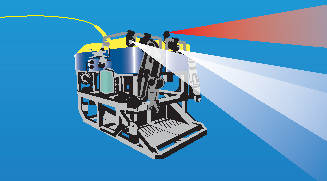
\includegraphics[width=\textwidth]{./pres/images/justJason}
        \end{center}
      \end{figure}
    \end{center}
  \column{.6\textwidth}

   \begin{itemize}
\item \alert<5>{ 6-DOF UV Model-Based Control (MBC)}
\item<1-4> 6-DOF UV Adaptive Model-Based Control (AMBC)
\item<1-4> Experimental Analysis: Thruster Dynamics and AMBC
\item<1-4> Experimental Evaluation: UV Two-Step AMBC
   \end{itemize}
\end{columns}
\vskip9pt
\uncover<1-4>{
\pause
Previous Research into UV Adaptive Model-Based Control (AMBC):
\pause
\begin{itemize}
\item Previous AMBC algorithms have been reported
\begin{itemize}
\item We report a novel AMBC algorithm which uses geometric control
  techniques to develop an error system which evolves on SE(3)
\end{itemize}
\pause
\item Previous AMBC experimental evaluations have been reported, but
  none have considered
\begin{itemize}
\item simultaneous motion in all DOF and
\item destabilizing effects of unmodeled thruster dynamics.
\end{itemize}
\end{itemize}}
\end{frame}

\subsection{UV Model-Based Control and Adaptive Extension}
\begin{frame}{UV {\it Non-Adaptive} Model-Based Control (MBC): Goal and State Representations}

\begin{columns}
      
  \column{.57\textwidth} MBC Goal: Design a control law ,
  {\color{green} $u$}, which uses the {\color{cyan} current vehicle
    state}, {\color{blue} a desired trajectory}, and {\color{red}
    known vehicle model} to provide asymptotically exact trajectory
  tracking.

      \begin{itemize}
      \item<2-> {\it actual} vehicle position {\color{cyan} ${^w_a}H$
        } and velocity {\color{cyan} ${^a}v_a$}
      \item<3-> {\it desired} vehicle position {\color{blue}
          ${^w_d}H$}, velocity {\color{blue} ${^d}v_d$}, and
        acceleration {\color{blue} ${^d}\dot{v}_d$}
      \item<4-> The vehicle parameters ${\color{red} M},~{\color{red}
          D},~{\color{red} g},~\text{and}~{\color{red} b}$ {\it are
          known}.  We will represent them using the parameter vector
        ${\color{red} \theta_{UV}}\in\rSp{241}$.
      \end{itemize} 

% \vspace*{10mm}
% \alt<1-4>{ 


% %      \vskip10pt
% }
% {

% }
    \column{.43\textwidth}
\uncover<5->{Error Coordinates}
\begin{itemize}
\item<5-6> \uncover<1-5>{$\Delta H={^w_d}H^{-1}{^w_a}H$} 
\begin{itemize}
\item<5-6> \alert<6>{$\Delta \psi=\log_{\SE3}\left(\Delta H \right)$}
\end{itemize}
\item<5-6> \alert<6>{$\Delta v={^a}v_a-{^a}v_d$}
\item<5> $\Delta \dot{H}=\Delta H\widehat{\Delta v}$
\begin{itemize}
\item $\Delta \dot{ \psi} = \hat{\mathcal{A}}^{-1}(\Delta \psi) \Delta v$
\end{itemize}
\item<5> $\Delta\dot{ v} = {^a}\dot{v}{_a}-{^a}\dot{v}{_d}+\ad_{\Delta v} {^a}v_d$
\item<5> $\hat{\mathcal{A}}^{-1}$ is the inverse of the se(3) velocity  
\end{itemize}


     \only<5->{
      \begin{center}
        \begin{figure}[htbp]  
          \begin{center}
  %          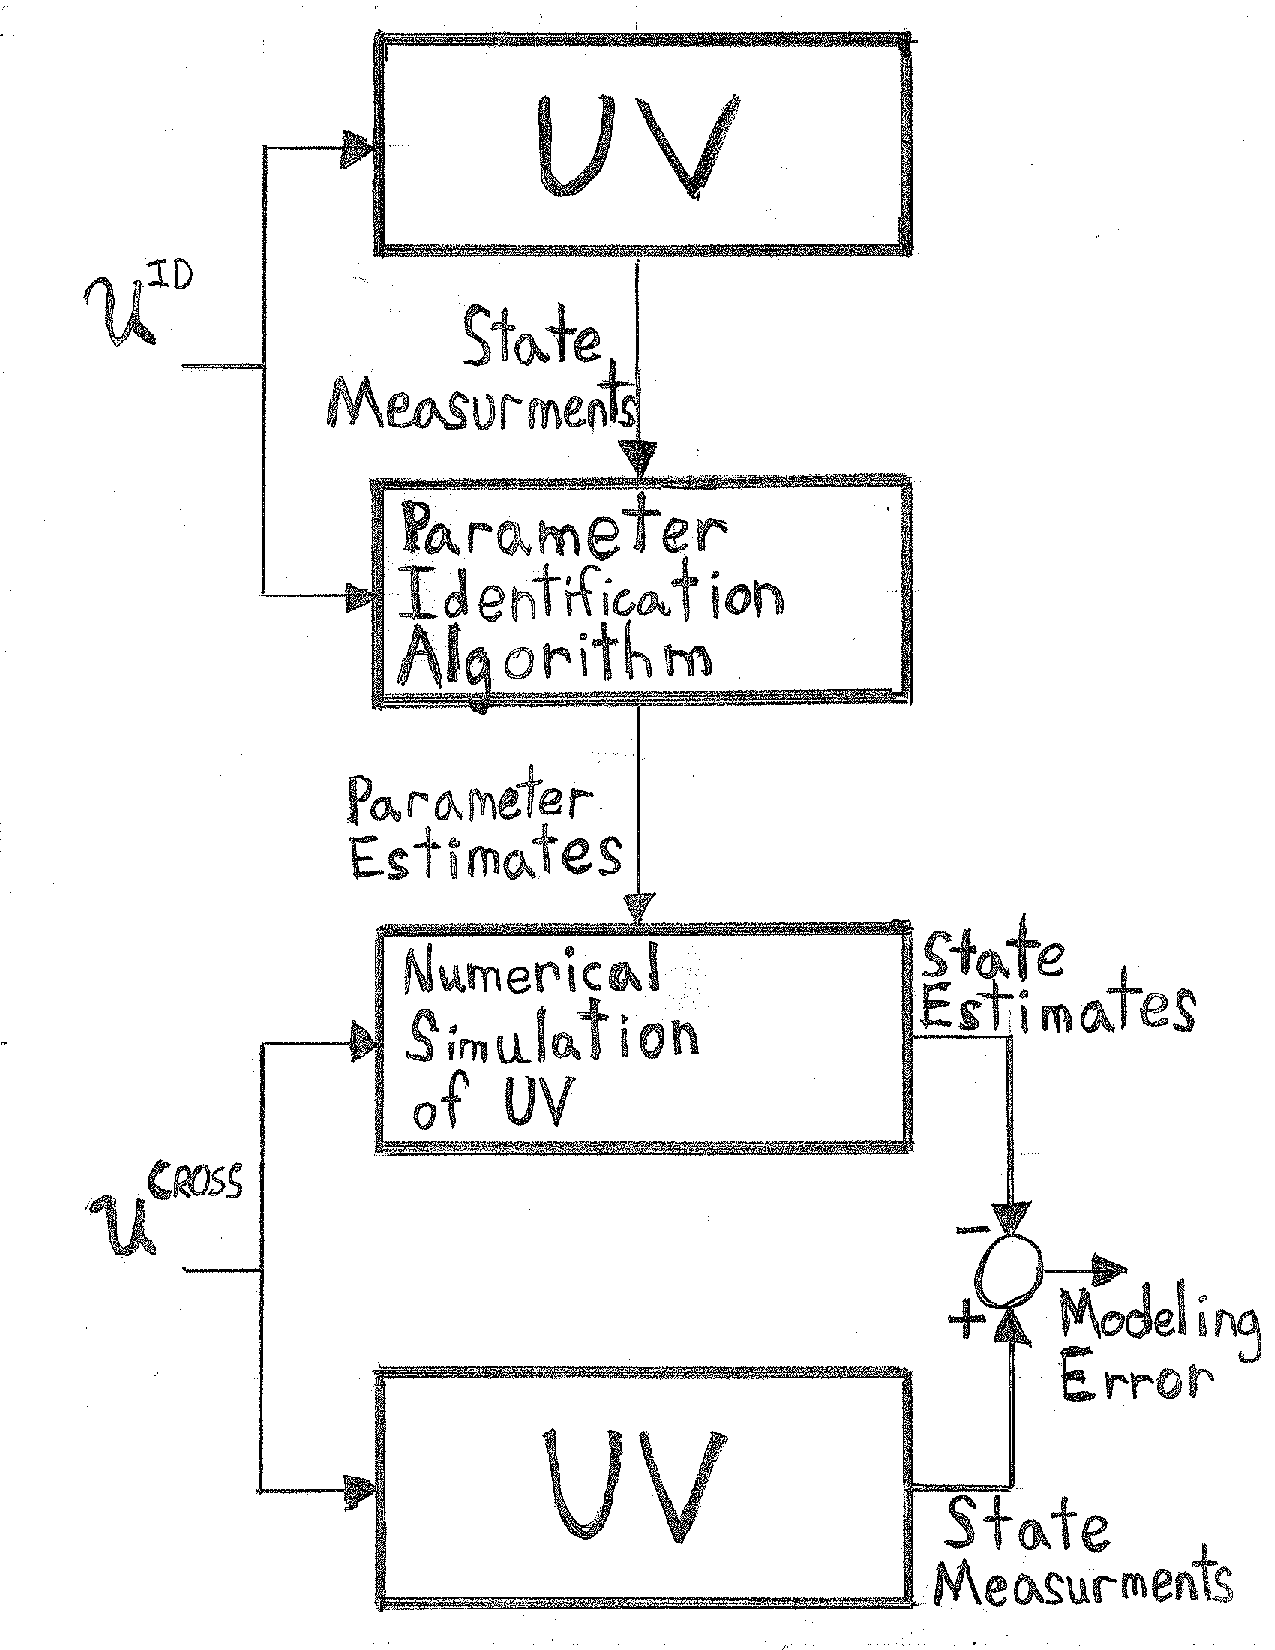
\includegraphics[width=50mm]{./pres/images/blockDiaSketch}
          \end{center}
        \end{figure}
      \end{center}    
      }
  \end{columns} 

\end{frame}



\begin{frame}[t]{Underwater Vehicle (non-adaptive) Model-Based Control}%{LS Model Identification}

%     \begin{columns}
%        \column{.3\textwidth}
% Plant Model:
%  \vskip10pt
% Control Law:
%  \vskip10pt
% Regressor:
%  \vskip10pt
%        \column{.7\textwidth}
%  \begin{align} 
%    \dot{H}(t)&={\color{cyan}H(t)}\widehat{{\color{cyan} v(t)}}
%    \nonumber \\
%    \alert{M}\dot{v}(t)&=\mathcal{H}(\alert{M}{\color{cyan} v(t)} ) {\color{cyan} v(t)}+
%    \sum_{i=1}^6 |{\color{cyan}v_i} |\alert{D_i}
%             {\color{cyan}v(t)}+
%    \mathcal{G}(\alert{g},\alert{b},{\color{cyan}H(t)})+\color{green}u(t)
%    \nonumber 
% \end{align}
% %
% \begin{equation*}
% u\left( {^w_a}H, {^a}v_a, {^w_d}H, {^d}v_d, {^d}\dot{v}_d\right)
% =-(k_p\hat{\mathcal{A}}^{-T}(\Delta \psi)+k_d\Delta v)+ 
% \MBCreg({^a}\dot{v}_d,\Delta v, {^a}v_d , {^w_a}H)\theta_{UV}
% \end{equation*}
% %
% \begin{equation*}
% \MBCreg({^a}\dot{v}_d,\Delta v, {^a}v_d , {^w_a}H)\theta_{UV} =
%     M{^a}\dot{v}_d - M\ad_{\Delta v}{^a}v_d -\ad_{{^a}v_a}^T M{^a}v_a
%     -\mathcal{D}({^a}v_a)-\mathcal{G}({^w_a}H)
% \end{equation*}
% \end{columns}


% {\small
% \begin{align} 
% \text{Plant Model:}\quad&\begin{cases}\dot{H}(t)&={\color{cyan}H(t)}\widehat{{\color{cyan} v(t)}}
%    \\
%    \alert{M}\dot{v}(t)&=\mathcal{H}(\alert{M}{\color{cyan} v(t)} ) {\color{cyan} v(t)}+
%    \sum_{i=1}^6 |{\color{cyan}v_i} |\alert{D_i}
%             {\color{cyan}v(t)}+
%    \mathcal{G}(\alert{g},\alert{b},{\color{cyan}H(t)})+\color{green}u(t)
%    \end{cases}
% \nonumber \\
% \text{Control Law:}\quad&u\left( {^w_a}H, {^a}v_a, {^w_d}H, {^d}v_d, {^d}\dot{v}_d\right)
% =-(k_p\hat{\mathcal{A}}^{-T}(\Delta \psi)+k_d\Delta v)+ 
% \MBCreg({^a}\dot{v}_d,\Delta v, {^a}v_d , {^w_a}H)\theta_{UV}
% \nonumber \\
% \text{Regressor:}\quad&\MBCreg({^a}\dot{v}_d,\Delta v, {^a}v_d , {^w_a}H)\theta_{UV} =
%     M{^a}\dot{v}_d - M\ad_{\Delta v}{^a}v_d -\ad_{{^a}v_a}^T M{^a}v_a
%     -\mathcal{D}({^a}v_a)-\mathcal{G}({^w_a}H)
% \nonumber 
% \end{align}
% }



{\small
\begin{align} 
\text{Plant Model:}\quad&\begin{cases}{^w_a}\dot{H}&={\color{cyan}{^w_a}H}\widehat{{\color{cyan} {^a}v_a}}
   \\
   \alert{M}{^a}\dot{v}_a&=\ad_{\color{cyan} {^a}v_a}^T\alert{M}{\color{cyan} {^a}v_a} +
   \sum_{i=1}^6 |{\color{cyan}{^a}v_{ai}} |\alert{D_i}
            {\color{cyan}{^a}v_a}+
   \mathcal{G}({\color{cyan}{^w_a}H})+\color{green}u
   \end{cases}
\nonumber \\
\text{Control Law:}\quad&u%\left( {^w_a}H, {^a}v_a, {^w_d}H, {^d}v_d, {^d}\dot{v}_d\right)
=-k_p\hat{\mathcal{A}}^{-T}(\Delta \psi)-k_d\Delta v+ 
\MBCreg\theta_{UV}
\nonumber \\
\MBCreg~ \text{such that:}\quad&\MBCreg\theta_{UV} =
    M{^a}\dot{v}_d - M\ad_{\Delta v}{^a}v_d -\ad_{{^a}v_a}^T M{^a}v_a
    -\sum_{i=1}^6 |{{^a}v_{ai}} |D_i
            {{^a}v_a}-\mathcal{G}({^w_a}H)
\nonumber 
\end{align}
\vskip7pt
\vskip7pt
\pause
This control law provides locally asymptotically stable trajectory tracking in the
sense of Lyapunov, i.e.  $\lim_{t\to \infty}\Delta \psi(t)=\vec{0}$
and $\lim_{t\to \infty}\Delta v(t)=\vec{0}$, if the following
conditions are met:

\begin{itemize}
\item the signals $\{{^w_d}H,{^d}v_d,{^d}\dot{v}_d
  \}\in\{\SE3,\realSpace{6},\realSpace{6}\}$ are continuous and bounded
\item $k_d,k_p\in\mathbb{R}_+$
\item $\|x(t_0)\|<\sqrt{
                  \frac{ {_\epsilon}\lambda_{12} }
                       { {_\epsilon}\lambda_1   }
                       } \pi$ 
\end{itemize}

\noindent where ${_\epsilon}\lambda_{1}$ and ${_\epsilon}\lambda_{12}$
are the largest and smallest eigenvalues, respectively, of
$\mathcal{M}_\epsilon\in\rSp{12\times 12}$ from the Lyapunov function.}


\end{frame}


\begin{frame}[t]{Outline of MBC Stability Analysis}
\begin{align}
\text{Error Dynamics:}\quad &\left[ \begin{array}{c}
     \Delta \dot{\psi}           \\
     \Delta \dot{v}              \\
\end{array} \right]=
\left[ \begin{array}{cc}
     0_{6\times 6}   & \hat{\mathcal{A}}^{-1}(\Delta \psi)             \\
     -k_p M^{-1}\hat{\mathcal{A}}^{-T}(\Delta \psi)   &  -k_d M^{-1}   \\
\end{array} \right]\left[ \begin{array}{c}
     \Delta \psi           \\
     \Delta v              \\
\end{array} \right]
\nonumber \\
\text{Lyapunov Fn:}\quad & 
V_1(t)=\frac{1}{2} \left[\begin{array}{cc}
   \Delta \psi^T & \Delta v^T
   \end{array} \right]
\left[ 
\begin{array}{cc}
  k_p\mathbb{I}_{6\times 6}  & \epsilon M         \\
  \epsilon M               &    M               \\
\end{array} \right]\left[ \begin{array}{c}
     \Delta \psi           \\
     \Delta v              \\
\end{array} \right]
\nonumber \\
\text{Lyap Derivative:}\quad & \dot{V}_1(t) \leq\frac{1}{2}\left[\begin{array}{cc}
   \|\Delta \psi\| & \|\Delta v\|
   \end{array} \right] 
  \left[\begin{array}{cc}
  -\epsilon 2 k_p  & \epsilon k_d    \\
 \epsilon k_d      &   \epsilon \lambda_1 c- 2k_d\\
  \end{array} \right] 
\left[\begin{array}{c}
   \|\Delta \psi\| \\ \|\Delta v\|
\end{array} \right] 
\nonumber
\end{align}

\pause

\begin{itemize}
\item For all $\epsilon\in\rSp{}_+$ such that
  $\epsilon\leq\min\left(\frac{4 k_p k_d}{2 \lambda_1 k_p c
      +k_d^2},\sqrt{\frac{k_p \lambda_6}{\lambda_1^{2}}} \right)$
  \\local asymptotically exact trajectory-tracking is proven
\item Several Properties for $\hat{\mathcal{A}}^{-1}(\Delta \psi)$
  required:
\begin{itemize}
\item $c$ is bound of $\|\hat{\mathcal{A}}^{-1}(\Delta \psi)\|$, local
  result required for bounded $c$
\item $\Delta\psi^T\left(\hat{\mathcal{A}}^{-T}+\hat{\mathcal{A}}^{-1}\right)\Delta
\psi=\Delta\psi^T\Delta\psi$
\end{itemize}
\item Facts proven in Appendices
\end{itemize}
\end{frame}


\begin{frame}{UV {\it Adaptive} Model-Based Control (AMBC): Goal and State Representations}

 
 

   \begin{columns}
      
     \column{.57\textwidth} AMBC Goal: Design a control law,
     {\color{green} $u$}, and parameter estimate update law, {\color{red}
       $\dot{\hat{\theta}}_{UV}$}, which uses the {\color{cyan}
       current vehicle state} and {\color{blue} desired trajectory}
     provide asymptotically exact trajectory tracking for a vehicle
     while all signals remain stable assuming the plant parameters are
     constant but unknown.  % \vskip10pt


      \begin{itemize}
     \item<2-> {\it actual} vehicle position {\color{cyan} ${^w_a}H$
        } and velocity {\color{cyan} ${^a}v_a$}
      \item<3-> {\it desired} vehicle position {\color{blue}
          ${^w_d}H$}, velocity {\color{blue} ${^d}v_d$}, and
        acceleration {\color{blue} ${^d}\dot{v}_d$}
      \item<4-> The vehicle parameters ${\color{red} M},~{\color{red}
          D},~{\color{red} g},~\text{and}~{\color{red} b}$ are {\it
          unknown}: we will use the parameter estimate vector
        ${\color{red} \hat{\theta}_{UV}}\in\rSp{241}$ and parameter
        error coordinates $\Delta\theta=\hat{\theta}_{UV}-\theta_{UV}$
      \end{itemize}
%
      \vspace*{10mm}
%

%
    \column{.43\textwidth} \only<2->{
      \begin{center}
        \begin{figure}[htbp]
          \begin{center}
  % 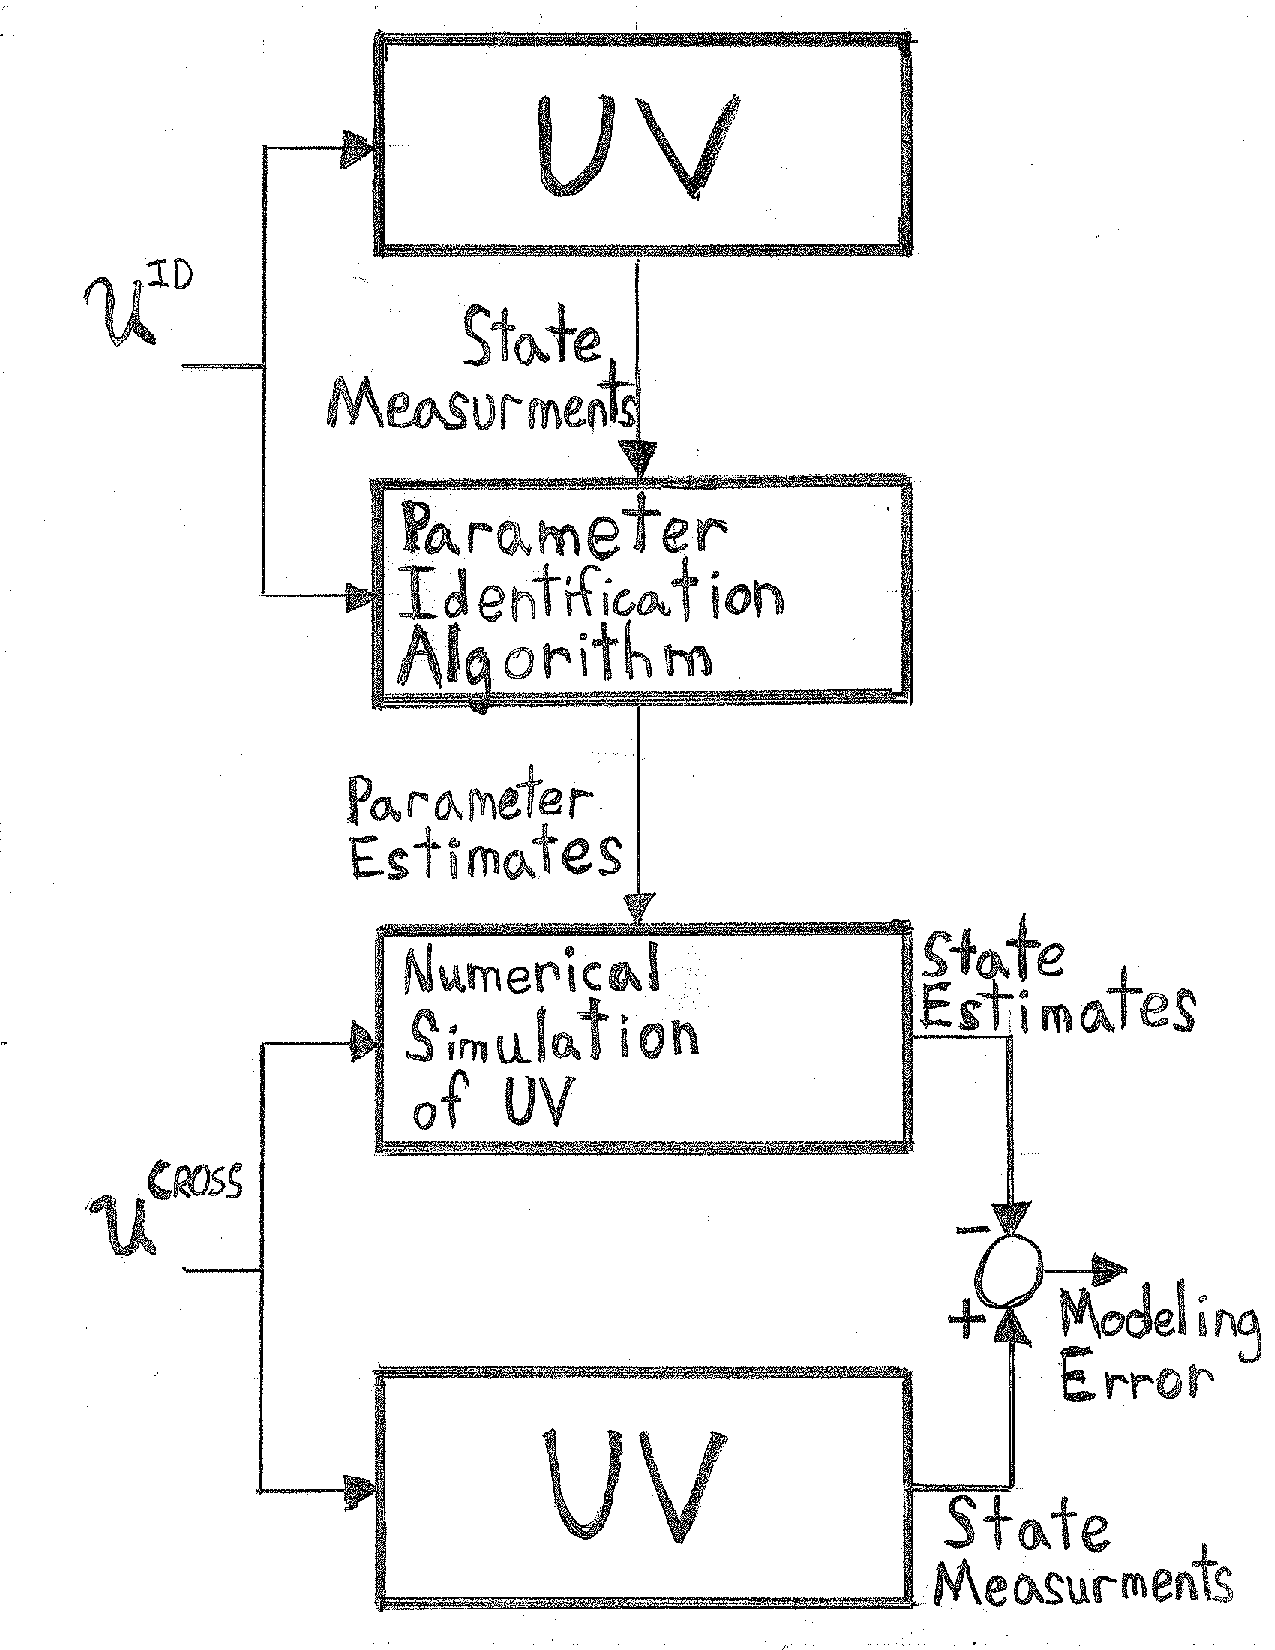
\includegraphics[width=50mm]{./pres/images/blockDiaSketch}
          \end{center}
        \end{figure}
      \end{center} }
  \end{columns}
\end{frame}



\begin{frame}[t]{Underwater Vehicle Adaptive Model-Based Control}

{\small
\begin{align} 
\text{Plant Model:}\quad&\begin{cases}\dot{H}(t)&={\color{cyan}H(t)}\widehat{{\color{cyan} v(t)}}
   \\
   \alert{M}\dot{v}(t)&=\ad_{\color{cyan} v(t)}^T\alert{M}{\color{cyan} v(t)} +
   \sum_{i=1}^6 |{\color{cyan}v_i} |\alert{D_i}
            {\color{cyan}v(t)}+
   \mathcal{G}(\alert{g},\alert{b},{\color{cyan}H(t)})+\color{green}u(t)
   \end{cases}
\nonumber \\
\text{Control Law:}\quad&u%\left( {^w_a}H, {^a}v_a, {^w_d}H, {^d}v_d, {^d}\dot{v}_d\right)
=-k_p\hat{\mathcal{A}}^{-T}(\Delta \psi)-k_d\Delta v+ 
\MBCreg\hat{\theta}_{UV}
\nonumber \\
\hat{\theta}_{UV}\text{ Update Law:}\quad&\dot{\hat{\theta}}
 =-K_\theta \MBCreg^T [\epsilon \Delta \psi +\Delta v]
\nonumber \\
\MBCreg~ \text{such that:}\quad&\MBCreg\hat{\theta}_{UV} =
    \hat{M}{^a}\dot{v}_d - \hat{M}\ad_{\Delta v}{^a}v_d -\ad_{{^a}v_a}^T \hat{M}{^a}v_a
    -\sum_{i=1}^6 |{{^a}v_{ai}} |\hat{D}_i
            {{^a}v_a}-\hat{\mathcal{G}}({^w_a}H)
\nonumber 
\end{align}


\pause This control law and parameter update law provide locally
asymptotically stable trajectory tracking and parameter estimates
which converge to constant values, i.e. $\lim_{t\to
  \infty}\dot{\hat{\theta}}(t)=0_{241 \times 1}$, if the MBC stability
conditions are met and:
%
\begin{itemize}
\item $K_\theta$ is SPD
\item $\epsilon<\min\left(\frac{4 k_p k_d}{2 \lambda_1 k_p c
    +k_d^2},\sqrt{\frac{k_p \lambda_6}{\lambda_1^{2}}} \right)$
\item $\sqrt{
      \frac{{_\epsilon}\lambda_1}{{_\epsilon}\lambda_{12}}\|x(t_0)\|^2+
      \frac{k_\theta}{{_\epsilon}\lambda_{12}}\|\Delta \theta(t_0)\|^2
       } <\pi$.
\end{itemize}
%
\noindent where $k_{\theta}=\frac{1}{\min{\eig{K_\theta}}}$ and
$\lambda_{1}$ and $\lambda_{6}$ are the largest and smallest
eigenvalues of $M$.}
\end{frame}



\begin{frame}[t]{Outline of AMBC Stability Analysis}
\begin{align}
\text{Error Dynamics:}\quad &\left[ \begin{array}{c}
     \Delta \dot{\psi}           \\
     \Delta \dot{v}              \\
\end{array} \right]=\hat{\mathbb{A}}(\Delta \psi)
\left[ \begin{array}{c}
     \Delta \psi           \\
     \Delta v              \\
\end{array} \right]+
\left[\begin{array}{c}
   0_{6\times 1}   \\ M^{-1}\MBCreg \Delta \theta
   \end{array} \right] 
\nonumber \\
\text{Lyapunov Fn:}\quad & 
V_2(t)=V_1(t)+ \frac{1}{2}\Delta\theta^T K_\theta^{-1} \Delta \theta
\nonumber \\
\text{Lyap Derivative:}\quad & \dot{V}_2(t) =\dot{V}_1(t)
%\leq\frac{1}{2}\left[\begin{array}{cc}
%   \|\Delta \psi\| & \|\Delta v\|
%   \end{array} \right] 
%  \left[\begin{array}{cc}
%  -\epsilon 2 k_p  & \epsilon k_d    \\
% \epsilon k_d      &   \epsilon \lambda_1 c- 2k_d\\
%  \end{array} \right] 
%\left[\begin{array}{c}
%   \|\Delta \psi\| \\ \|\Delta v\|
%\end{array} \right] 
\nonumber
\end{align}

\begin{itemize}
\item  Stability analysis builds off MBC stability analysis: $\hat{\mathbb{A}}(\Delta \psi)=\left[ \begin{array}{cc}
     0_{6\times 6}   & \hat{\mathcal{A}}^{-1}(\Delta \psi)             \\
     -k_p M^{-1}\hat{\mathcal{A}}^{-T}(\Delta \psi)   &  -k_d M^{-1}   \\
\end{array} \right]$
\pause
\item As with MBC, for all $\epsilon\in\rSp{}_+$ such that $\epsilon\leq\min\left(\frac{4 k_p k_d}{2 \lambda_1 k_p c
    +k_d^2},\sqrt{\frac{k_p \lambda_6}{\lambda_1^{2}}} \right)$ \\ local asymptotically exact trajectory-tracking is proven.
\item In addition to MBC conditions on initial state of the system, now conditions on the initial parameter error
      are required to maintain the bounded $c$.
\end{itemize}
\end{frame}

